\part{MicroRTS}
\frame{\partpage}

\begin{frame}{MicroRTS competition}
	\begin{itemize}
		\pause\item This should be your main focus (for COMP250) from now on
		\pause\item Fork the repository at \url{https://github.com/falmouth-games-academy/comp250-bot}
			and follow the instructions
		\pause\item Look at the example bots in the \texttt{microrts} project
			\begin{itemize}
				\pause\item Start with the ``rush'' bots in \texttt{ai.abstraction}
				\pause\item Move on to search-based AI: \texttt{ai.minimax.RTMiniMax.RTMiniMax},
					\texttt{ai.mcts.naivemcts.NaiveMCTS}, ...
				\pause\item Use these samples as a basis to create your own AI
			\end{itemize}
	\end{itemize}
\end{frame}

\begin{frame}{Playing the game}
    \begin{center}
        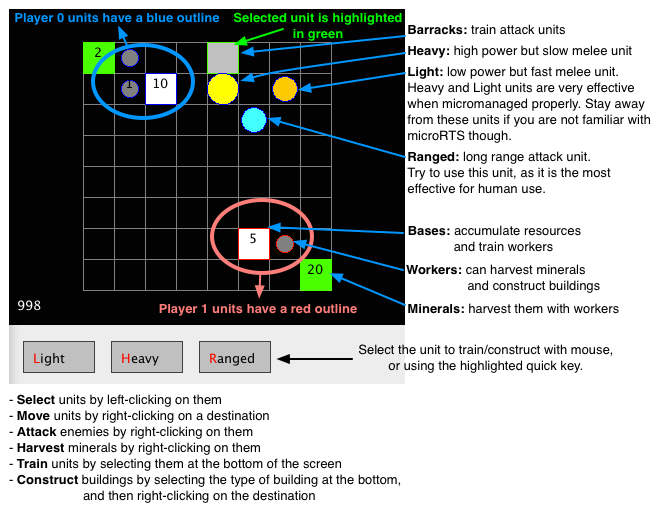
\includegraphics[height=0.8\textheight]{microrts_game}
    \end{center}
\end{frame}

\begin{frame}{MicroRTS}
    \begin{itemize}
        \pause\item \textbf{Workers} can harvest \textbf{minerals} and build \textbf{bases} and \textbf{barracks}
        \pause\item \textbf{Bases} can train \textbf{workers}
        \pause\item \textbf{Barracks} can train \textbf{attack units}
        \pause\item \textbf{Attack units}: light, heavy, ranged (workers can also attack)
    \end{itemize}
\end{frame}

\begin{frame}{MicroRTS bot}
    \begin{itemize}
        \pause\item \lstinline{getAction} is called every game tick
        \pause\item Assign \textbf{actions} to each of the player's units (including buildings)
        \pause\item Two levels to work at:
            \begin{itemize}
                \pause\item Basic actions up, down, left, right, attack, etc.
                \pause\item \lstinline{AbstractionLayerAI}: higher-level actions with built-in pathfinding, e.g.\
                    \lstinline{move}, \lstinline{build}, \lstinline{attack} etc.
            \end{itemize}
    \end{itemize}
\end{frame}

\begin{frame}{Example bots}
\end{frame}
